\documentclass[12pt]{article}

%%%%%%%%%%%%%%%%%%%%%%%%%%%%%%%%%%%%%%%%%%%%%%%%%%%%%%%%%%%%

\title{LaTeX Demo}
\author{Nathan Schill}
\date{\today}

%%%%%%%%%%%%%%%%%%%%%%%%%%%%%%%%%%%%%%%%%%%%%%%%%%%%%%%%%%%%

\PassOptionsToPackage{style=alphabetic}{biblatex}

\newcommand{\commandprependpath}{../}
\usepackage{../style}

\addbibresource{../my-references.bib}

% Miscellaneous
\newcommand{\scrL}{\mathscr{L}}


\graphicspath{{figures/}}

\begin{document}

\maketitle

%%%%%%%%%%%%%%%%%%%%%%%%%%%%%%%%%%%%%%%%%%%%%%%%%%%%%%%%%%%%

Behold, content.

And now, a citation \cite{neweyModelDiscoveryFly2024}.

\begin{figure}[h]
  \centering
  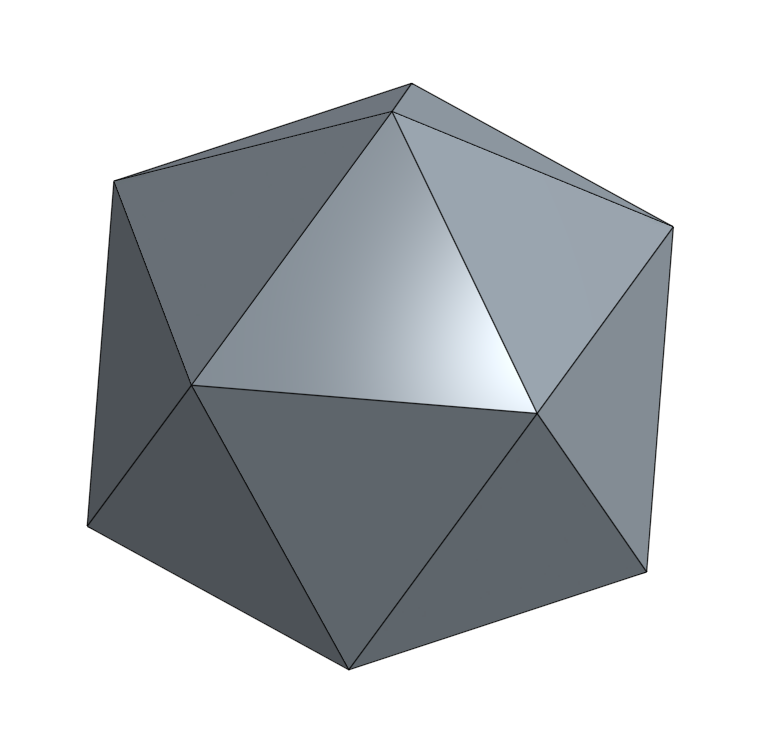
\includegraphics[width=0.4\textwidth]{icosahedron.png}
  \caption{Here, an icosahedron.}
  \label{fig:icosahedron}
\end{figure}

A reference to \cref{fig:icosahedron}.

Taylor series!
\begin{alignat*}{4}
  u(x)
  &= u(x_0)
  &&+ u'(x_0)(x - x_0)
  &&+ \frac{u''(x_0)}{2!}(x - x_0)^2 \\
  &+ \frac{u'''(x_0)}{3!}(x - x_0)^3
  &&+ \frac{u^{(4)}(x_0)}{4!}(x - x_0)^4
  &&+ \frac{u^{(5)}(x_0)}{5!}(x - x_0)^5 \\
  &+ \frac{u^{(6)}(x_0)}{6!}(x - x_0)^6
  &&+ \frac{u^{(7)}(x_0)}{7!}(x - x_0)^7
  &&+ \frac{u^{(8)}(\xi)}{8!}(x - x_0)^8
\end{alignat*}

\section*{Paired delimiter commands}

The following demonstrates paired delimiter commands from \texttt{common.tex}, showing how they automatically resize with larger content.

\subsection*{Parentheses}

\texttt{\textbackslash paren*\{\textbackslash frac\{a\}\{b\}\}} produces:
\[
  \paren*{\frac{a}{b}}
\]

\subsection*{Square Brackets}

\texttt{\textbackslash bbrack*\{\textbackslash frac\{a\}\{b\}\}} produces:
\[
  \bbrack*{\frac{a}{b}}
\]

\subsection*{Curly Braces}

\texttt{\textbackslash bbrace*\{\textbackslash frac\{a\}\{b\}\}} produces:
\[
  \bbrace*{\frac{a}{b}}
\]

\subsection*{Absolute Value}

\texttt{\textbackslash abs*\{\textbackslash frac\{a\}\{b\}\}} produces:
\[
  \abs*{\frac{a}{b}}
\]

\subsection*{Norm}

\texttt{\textbackslash norm*\{\textbackslash frac\{a\}\{b\}\}} produces:
\[
  \norm*{\frac{a}{b}}
\]

\subsection*{Inner Product}

\texttt{\textbackslash inpr*\{\textbackslash frac\{a\}\{b\}, c\}} produces:
\[
  \inpr*{\frac{a}{b}, c}
\]

%%%%%%%%%%%%%%%%%%%%%%%%%%%%%%%%%%%%%%%%%%%%%%%%%%%%%%%%%%%%

\appendix

\newpage
\printbibliography

\end{document}
